\documentclass[a4paper,12pt]{article} % Tipo de documento y tamaño de letra.
\usepackage[utf8]{inputenc} % Para que reconozca caracteres especiales como tildes.
\usepackage[spanish]{babel} % Para definir el idioma y el formato de fechas en español.
\usepackage{amsmath, amssymb} % Paquetes para símbolos y ecuaciones avanzadas (Para hacer una ecuación con un recuadro).
\usepackage{ragged2e} % Para justificar textos.
\usepackage{multicol} % Para crear columnas.
\usepackage{slashed} % Para generar números o variables canceladas (Una línea diagonal sobre el número o variable)
\usepackage{graphicx} % Paquete para poner graficas.
\usepackage{float} % Para poder dejar la imagen en un punto fijo del documento.
\usepackage{longtable} % Para tablas largas.
\usepackage{cancel} % Para hacer cancelaciones en medio de operaciones.
\usepackage{xcolor} % Para el color y esas cosas.
\usepackage{apacite} % Paquete para citas APA.
\usepackage{fancyhdr} % Para personalizar encabezados y pies de página.
\usepackage{geometry} % Para ajustar márgenes.
\usepackage{setspace} % Para ajustar el interlineado.
\usepackage{natbib}  % Para manejar las citas y que no queden pegadas y feas :P.
\usepackage{hyperref} % Para que los enlaces sean clickeables.


\pagestyle{fancy}
\fancyhf{} % Limpia encabezados y pies de página predeterminados
\fancyhead[L]{\textbf{LABORATORIO}} % Encabezado izquierdo
\fancyhead[R]{\textbf{ESTADÍSTICA}} % Encabezado derecho
\fancyfoot[C]{\thepage} % Número de página en el centro del pie

\geometry{headheight=12.96115pt, top=1in, bottom=1in, left=1in, right=1in}
\begin{document}


\begin{figure}[H] 
    \centering
    
\includegraphics[width=0.5\textwidth]{Unir.jpg} 
\end{figure}

\vspace{\baselineskip}

% Ajustamos manualmente todo ;)
\begin{center}
    \textbf{\Large PRODUCCIÓN ENERGÉTICA Y CONSUMO } \\[0.3cm]
    \vspace{\baselineskip}
    \textbf{Liz Ángel Núñez Torres} \\[0.4cm]
    \textbf{Grado en Física} \\[0.4cm]
    \textbf{Universidad Internacional de La Rioja} \\[0.4cm]
    \textbf{21 de marzo de 2025}
\end{center}


\newpage
\tableofcontents

\newpage



\section{Cita y problemas estadísticos.}

\begin{justify}
El consumo y producción energética \cite{owid-energy-production-consumption}.
\end{justify}

\begin{itemize}
    \item ¿Es el consumo energético promedio diferente de la producción energética promedio? % Usamos la media yuna prueba t de Student para comparar las medias de ambos datasets.
    \item ¿Cuál es la dispersión de los datos en el consumo y la producción energética? % Calcular la desviación estándar para ambos datasets.
\end{itemize}

\section{Referencias relevantes.}

\begin{justify}
    Artículos similares \cite{Consumption-Energy} y \cite{renewable-energy}.
\end{justify}

\section{Construir un algoritmo en R.}

\begin{justify}
    El algoritmo que usamos en nuestro archivo \textbf{.R} para responder a nuestras dos preguntas es:
\end{justify}

\begin{enumerate}
    \item \textbf{Importar datos:} Se cargan en nuestro archivo los datasets \textbf{Elec\_generation} y \textbf{Elec\_consumption}.
    \item \textbf{Análisis de medias:} Se calculan las medias de consumo y producción y se realiza una prueba t para compararlas.
    \item \textbf{Medición de dispersión:} Se calcula la varianza y la desviación estándar para ambos conjuntos de datos.
\end{enumerate}

\section{Bases de datos.}

\begin{justify}
    Usamos dos datasets o bases de datos.
\end{justify}

\begin{itemize}
    \item Consumo energético (Global Energy Consumption (2000-2024))\(\Rightarrow\) \cite{Data-set}
    \item Producción energética. (Electricity generation, 2023) \(\Rightarrow\) \cite{owid-energy-production-consumption}.
\end{itemize}

\section{Fotografía de los datos.}



\begin{figure}[H]

    \centering
    \begin{minipage}{0.30\textwidth} 
        \centering
        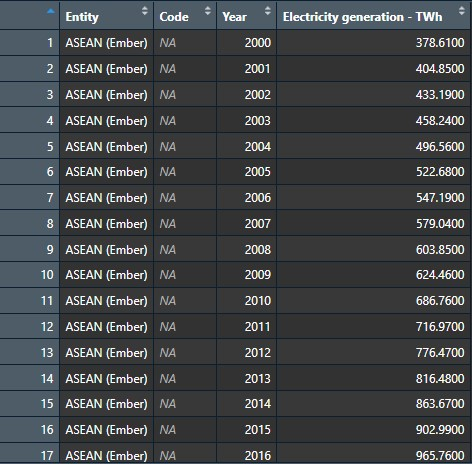
\includegraphics[width=\textwidth]{generation.jpg} 
        \caption{DataFrame sobre la generación energética.}
    \end{minipage}
    \hfill 
    \begin{minipage}{0.48\textwidth}  
        \centering
        \includegraphics[width=\textwidth]{consumption.jpg}
        \caption{DataFrame sobre el consumo energético.}
    \end{minipage}
    
\end{figure}

\begin{justify}
    Con los datos presentados podemos relacionar variables tales como ``Electricity generation'' y ``Total Energy Consumption''
    para obtener la media consumida y producida.
\end{justify}

\begin{justify}
    Con las mismas variables podemos obtener la varianza y la desviación estándar, donde la dispersión de nuestros datos y la distribución de los mismos generan las herramientas
    necesarias para comprender porque existe más o menos consumo/generación energética.
\end{justify}

\section{Informes gráficos.}


\begin{figure}[H]

    \centering
    \begin{minipage}{0.48\textwidth} 
        \centering
        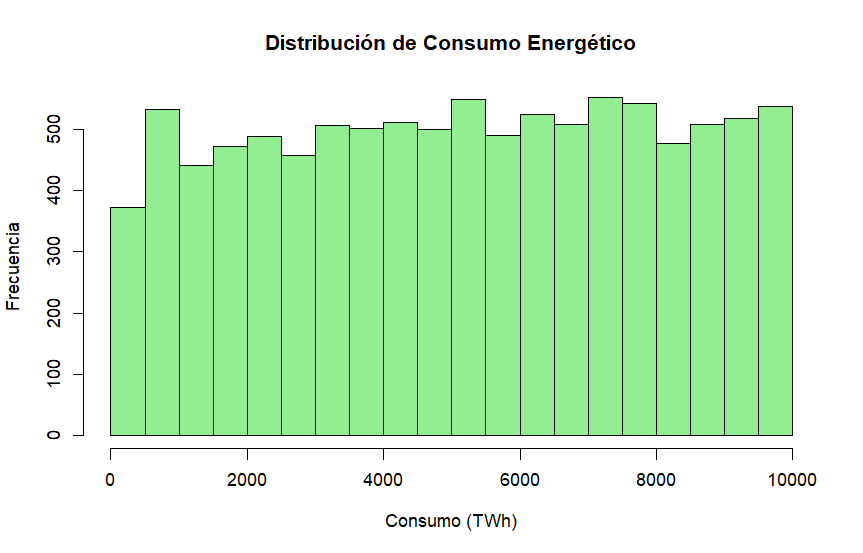
\includegraphics[width=\textwidth]{Consumo_Ener.png} 
    \end{minipage}
    \hfill 
    \begin{minipage}{0.48\textwidth}  
        \centering
        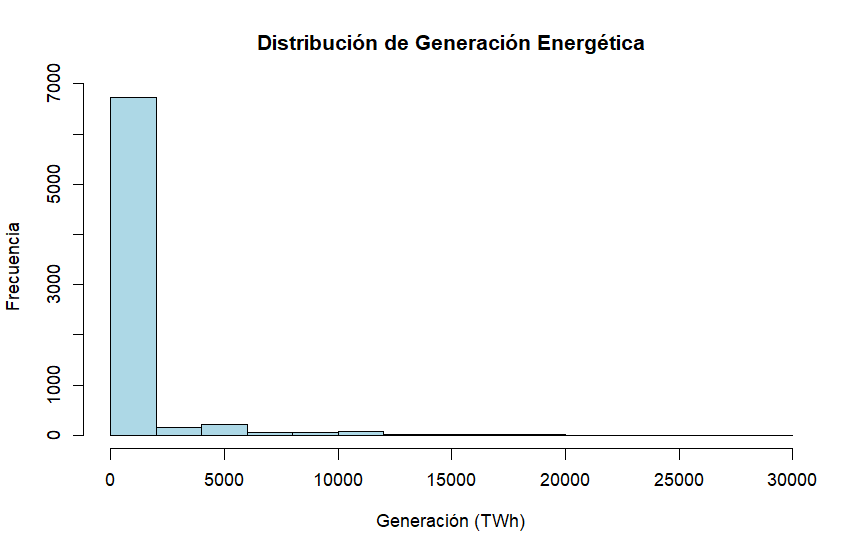
\includegraphics[width=\textwidth]{Generacio_ener.png}
    \end{minipage}
    
\end{figure}

\begin{figure}[H]
    \centering
    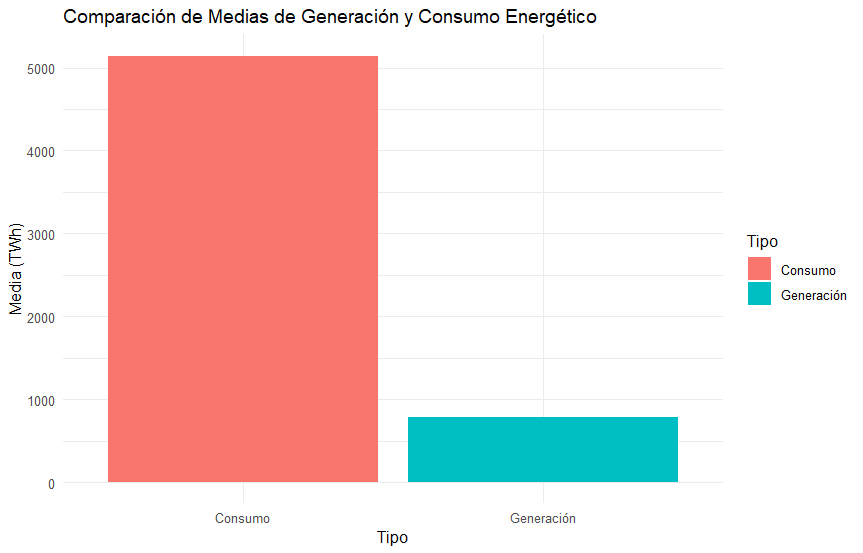
\includegraphics[width=0.8\textwidth]{Medias.png}
\end{figure}


\section{Conclusiones.}

\begin{justify}
    Los datos presentados en los gráficos de distribución y comparación de medias muestran una brecha
    significativa entre la generación y el consumo energético, generando un impacto directo en la calidad de vida de la población y en los costos energéticos.
    Para abordar este problema, es crucial implementar inversión en energías renovables y mejoras en la eficiencia energética, 
    especialmente en regiones donde el desequilibrio es más pronunciado.

\end{justify}

\newpage


% Aquí ajustamos y usamos las referencias y citas del archivo .bib.
\setlength{\bibsep}{12pt} % Ajusta la separación entre referencias
\bibliographystyle{apacite} % Estilo APA
\bibliography{citas} % Archivo de referencias


\section{Calificación/Observaciones.}

\begin{figure}[H]
    \centering
    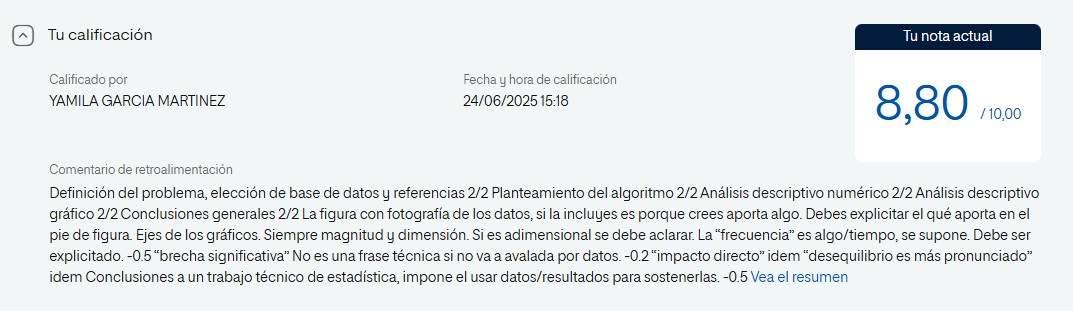
\includegraphics[width=1.1 \textwidth]{calificacion.jpg}
\end{figure}






\end{document}